\documentclass{article}
\usepackage[utf8]{inputenc}
\usepackage{tikz}
\usepackage{amsmath}
\usetikzlibrary{positioning}

\begin{document}

%------------------------------------------------------------------------------
% QSPK

\begin{figure}
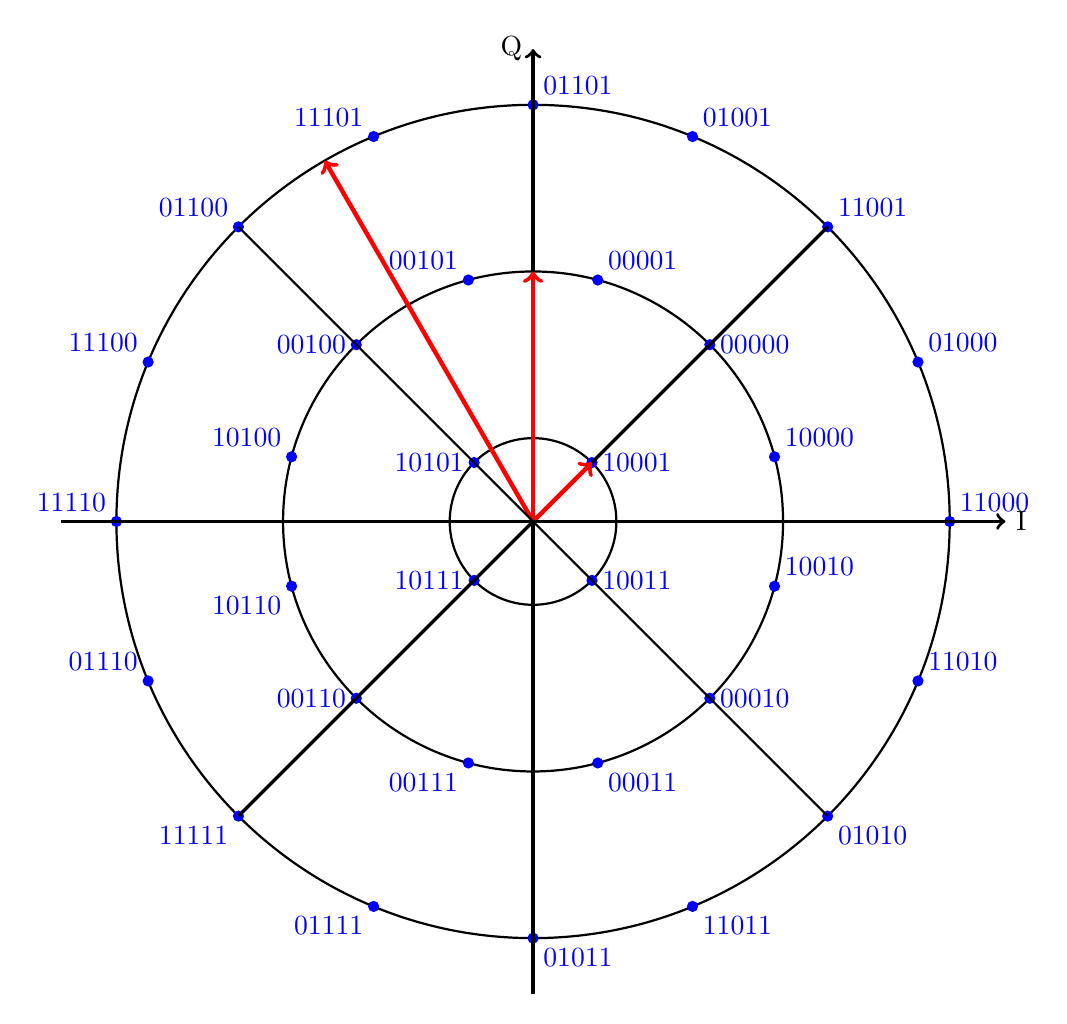
\begin{tikzpicture}[thick,scale=0.4]
%---------------------Inner Most Circle------------------%
\draw[thick](0,0) circle (2.64575131);
\filldraw [blue] (2.64575131*0.707106781,2.64575131*0.707106781) circle (4pt) node[anchor=west] {10001};
\filldraw [blue] (2.64575131*-0.707106781,2.64575131*0.707106781) circle (4pt) node[anchor=east] {10101};
\filldraw [blue] (2.64575131*-0.707106781,2.64575131*-0.707106781) circle (4pt) node[anchor=east] {10111};
\filldraw [blue] (2.64575131*0.707106781,2.64575131*-0.707106781) circle (4pt) node[anchor=west] {10011};
%--------------------------------------------------------%

%---------------------Middle Circle------------------%
\draw[thick](0,0) circle (3*2.64575131);
%-------------------Q1-------------------------%
\filldraw [blue] (3*2.64575131*0.965925826,3*2.64575131*0.258819045) circle (4pt) node[anchor=south west] {10000};
\filldraw [blue] (3*2.64575131*0.707106781,3*2.64575131*0.707106781) circle (4pt) node[anchor= west] {00000};
\filldraw [blue] (3*2.64575131*0.258819045,3*2.64575131*0.965925826) circle (4pt) node[anchor=south west] {00001};

%-------------------Q2-------------------------%
\filldraw [blue] (3*2.64575131*-0.258819045,3*2.64575131*0.965925826) circle (4pt) node[anchor=south east] {00101};
\filldraw [blue] (3*2.64575131*-0.707106781,3*2.64575131*0.707106781) circle (4pt) node[anchor=east] {00100};
\filldraw [blue] (3*2.64575131*-0.965925826,3*2.64575131*0.258819045) circle (4pt) node[anchor=south east] {10100};

%-------------------Q3-------------------------%
\filldraw [blue] (3*2.64575131*-0.965925826,3*2.64575131*-0.258819045) circle (4pt) node[anchor=north east] {10110};
\filldraw [blue] (3*2.64575131*-0.707106781,3*2.64575131*-0.707106781) circle (4pt) node[anchor=east] {00110};
\filldraw [blue] (3*2.64575131*-0.258819045,3*2.64575131*-0.965925826) circle (4pt) node[anchor=north east] {00111};

%-------------------Q4-------------------------%
\filldraw [blue] (3*2.64575131*0.258819045,3*2.64575131*-0.965925826) circle (4pt) node[anchor=north west] {00011};
\filldraw [blue] (3*2.64575131*0.707106781,3*2.64575131*-0.707106781) circle (4pt) node[anchor=west] {00010};
\filldraw [blue] (3*2.64575131*0.965925826,3*2.64575131*-0.258819045) circle (4pt) node[anchor=south west] {10010};
%--------------------------------------------------------%

%----------------------------Outer Most Circle--------------------%
\draw[thick](0,0) circle (5*2.64575131);

%-------------------Q1-------------------------%
\filldraw [blue] (5*2.64575131,0) circle (4pt) node[anchor=south west] {11000};
\filldraw [blue] (5*2.64575131*0.923879533,5*2.64575131*0.382683432) circle (4pt) node[anchor=south west] {01000};
\filldraw [blue] (5*2.64575131*0.707106781,5*2.64575131*0.707106781) circle (4pt) node[anchor=south west] {11001};
\filldraw [blue] (5*2.64575131*0.382683432,5*2.64575131*0.923879533) circle (4pt) node[anchor=south west] {01001};

%-------------------Q2-------------------------%
\filldraw [blue] (0,5*2.64575131) circle (4pt) node[anchor=south west] {01101};
\filldraw [blue] (5*2.64575131*-0.382683432,5*2.64575131*0.923879533) circle (4pt) node[anchor=south east] {11101};
\filldraw [blue] (5*2.64575131*-0.707106781,5*2.64575131*0.707106781) circle (4pt) node[anchor=south east] {01100};
\filldraw [blue] (5*2.64575131*-0.923879533,5*2.64575131*0.382683432) circle (4pt) node[anchor=south east] {11100};

%-------------------Q3-------------------------%
\filldraw [blue] (5*-2.64575131,0) circle (4pt) node[anchor=south east] {11110};
\filldraw [blue] (5*2.64575131*-0.923879533,5*2.64575131*-0.382683432) circle (4pt) node[anchor=south east] {01110};
\filldraw [blue] (5*2.64575131*-0.707106781,5*2.64575131*-0.707106781) circle (4pt) node[anchor=north east] {11111};
\filldraw [blue] (5*2.64575131*-0.382683432,5*2.64575131*-0.923879533) circle (4pt) node[anchor=north east] {01111};

%-------------------Q4-------------------------%
\filldraw [blue] (0,-5*2.64575131) circle (4pt) node[anchor=north west] {01011};
\filldraw [blue] (5*2.64575131*0.382683432,5*2.64575131*-0.923879533) circle (4pt) node[anchor=north west] {11011};
\filldraw [blue] (5*2.64575131*0.707106781,5*2.64575131*-0.707106781) circle (4pt) node[anchor=north west] {01010};
\filldraw [blue] (5*2.64575131*0.923879533,5*2.64575131*-0.382683432) circle (4pt) node[anchor=south west] {11010};
%--------------------------------------------------------%

\draw[red,ultra thick,->] (0,0) -- (2.64575131*0.707106781,2.64575131*0.707106781);
\draw[red,ultra thick,->] (0,0) -- (5*2.64575131*-0.5,5*2.64575131*0.866025404);
\draw[red,ultra thick,->] (0,0) -- (0,3*2.64575131);
\draw[black,very thick,->] (-15,0) -- (15,0) node[anchor=west] {I};
\draw[black,very thick] (0,-15) -- (0,0) ;
\draw[black,very thick] (2.64575131*0.707106781,2.64575131*0.707106781) -- (5*2.64575131*0.707106781,5*2.64575131*0.707106781) ;
\draw[black,very thick] (0,0) -- (5*2.64575131*-0.707106781,5*2.64575131*-0.707106781) ;
\draw[black,thick] (5*2.64575131*-0.707106781,5*2.64575131*0.707106781) -- (5*2.64575131*0.707106781,5*2.64575131*-0.707106781) ;
\draw[black,very thick,->] (0,3*2.64575131) -- (0,15) node[anchor=east] {Q};
\end{tikzpicture}
\end{figure}

\begin{equation*}
X_k \in \cbrak{X}=
\begin{cases}
r_1 e^{j\brak{\phi_1+\frac{2\pi}{4}n}}& n=0,\dots,3\\
r_2 e^{j\brak{\phi_2+\frac{2\pi}{12}n}}& n=0,1,\dots,11\\
r_3 e^{j\brak{\phi_3+\frac{2\pi}{16}n}}& n=0,1,\dots,16
\end{cases}
\end{equation*}
%------------------------------------------------------------------------------

\end{document}